\chapter[Referencial Teórico]{Referencial Teórico}

\section{USO DAS TECNOLOGIAS NA EDUCAÇÃO}

As tecnologias chegaram as escolhas, segundo \citeonline{moran}, apesar da resistência institucional, as mudanças são necessárias. As empresas estão muito ativas na educação online e buscam agilidade das universidades, flexibilização e rapidez na educação continuada. Os avanços na educação à distância com a Internet é bem notável. A Internet retirou a isolação da educação a distância, de atraso ou de ensino de segunda classe. A interconectividade que a Internet desenvolveu nesses últimos anos, começou a revolucionar a forma de ensinar e aprender.
\par
Em um artigo publicado na revista Veja, chamado "O computador não educa ensina" por \citeonline{veja-educacao}, pergunta como as escolas irão fazer uso do computador um instrumento para mudar a velha escola, praticamente congelada no tempo desde o século XIX? A publicação mostra experiência de países que utilizam essa ferramenta no processo de ensino aprendizagem, como é o caso do Japão, o autor diz: "Estudar em rede lá se tornou uma febre". No Japão as escolas estão ensinando em rede, e isso abre uma nova dimensão no exercício intelectual, em que as crianças são incentivadas a desenvolver com rapidez de raciocínio para dar respostas on-line e a expor ideias para centenas de colegas virtuais, ajudando também no quesito de trabalho em equipe do aluno.
\par
Para \citeonline{goncalves}  a tecnologia é muito mais do que apenas equipamentos, máquinas e computadores. A organização só funciona a partir da operação de dois sistemas que dependem um do outro, o sistema técnico, formado pelas técnicas e ferramentas usadas para realizar cada tarefa, e o sistema social, com suas necessidades, expectativas, e sentimentos sobre o trabalho. Os dois sistemas são usados de forma otimizada quando os requisitos da tecnologia e as necessidades das pessoas são atendidos conjuntamente. Dessa forma é possível distinguir entre tecnologia(conhecimento) e sistema técnico (combinação de máquinas e métodos para obter um resultado desejado).
\par
Seguindo o pensamento de Gonçalves, um artigo da Gazeta do Povo por \citeonline{juliana-gazeta}, afirma que "O computador não ensina nada sozinho", assim como a presença de ou não de um laboratório de informática, não quer dizer muita coisa sobre a qualidade de ensino de uma escola, mais que um bom planejamento faz a diferença, complementa também que pouco adianta usar o computador em sala seguindo uma metodologia tradicional, como uma ferramenta para fazer apenas cópias de texto, pois isso pode ser feito com lápis e caderno.

\section{EDUCAÇÃO À DISTÂNCIA (EAD)}

\citeonline{moran-ead} descreve a Educação a Distância como um processo de ensino-aprendizagem, mediado por tecnologias, onde professores e alunos estão separados espacial e/ou temporalmente.
\par
O conceito de distância em EaD deve ser entendida como uma separação espacial (geográfica/local) entre participantes do processo educacional, sejam alunos ou professores. Quando o estudo ocorre pela internet, alunos e professores podem estar em lugares diferentes, e ainda assim possam acessar o curso e os materiais e recursos educativos em momentos distintos.
\par
\citeonline[p.~3]{vilacca} salienta que as formas de distância podem gerar incompreensões, criando preconceitos em relação a EaD. A distância não implica necessariamente em divergência temporal (cronológica), alunos e professores podem estar em locais diferentes, participando de forma síncrona de uma mesma atividade, como por \textit{chat}. \apud[p.~3]{vilacca}{valente}  destacam também que o distanciamento físico entre os participantes "não implica em distanciamento humano", os autores descrevem também que a EaD, "possibilita a manipulação do espaço e do tempo em favor da educação." \apud[p.~3]{vilacca}{valente}.
\par
O conceito de curso e de aula também é um pouco diferente do que entendemos hoje, de uma aula com espaço e tempo determinados, com a internet por exemplo, esse tempo e espaço fica cada vez mais flexível. Esse processo é descrito por \citeonline[p.~2]{moran-ead} em seu artigo:
\begin{citacao}
  O professor continuará "dando aula", e enriquecerá esse processo com as possibilidades que as tecnologias interativas proporcionam: para receber e responder mensagens dos alunos, criar listas de discussão e alimentar continuamente os debates e pesquisas com textos, páginas da internet, até mesmo foram do horário específico da aula.
\end{citacao}
\par
Dessa forma o Ensino a Distância também pode ser usado como um complemento a uma aula presencial tradicional, enriquecendo-a.
\par
O EaD é uma forma do aluno aprender a distância, por vários meios, como correspondências, televisão, radio e internet. Com a união do Ensino a distância com a \textit{Internet}, surgiu um novo termo conhecido como \textit{e-Learning}, uma modalidade de aprendizagem baseada na Internet.

\newpage
\subsection{\textit{ELETRONIC LEARNING (E-LEARNING)}}
Segundo \citeonline{rodrigues} a \textit{e-Learning} é uma modalidade de ensino a distância que possibilita a auto aprendizagem, com recursos didáticos sistematicamente organizados, apresentados em diferentes suportes tecnológicos de informação, utilizados de forma isolada ou combinada através da internet.
\par
\citeonline{Felipini} acrescenta que a \textit{e-Learning} é basicamente um sistema em um servidor, que transmite através da Internet ou Intranet, informações e instruções aos alunos para agregar um conhecimento especifico. As etapas de ensino no \textit{e-Learning} são pré-programadas, podem ou não ser divididas em módulos e para o ensino, podem ser usados diversos recursos como e-mail, textos, imagens, texto, \textit{chat}, \textit{links} de informação externa, vídeos e teleconferências.
\par
O \textit{e-learning} também pode ser definido como um método de ensino a distância que usa novas tecnologias multimédia e Internet para promover a qualidade da formação, facilitando assim o acesso a recursos e serviços, assim como trocas de informações entre os diversos intervenientes envolvidos. \cite{spi}.
\par
\cite[p.~3]{barbosa} descreve as necessidades de um sistema de \textit{e-Learning}:
\begin{citacao}
  Para que seja possível uma aula/formação, com o modelo de e-Learning, é necessário que o e-tutor disponibilize os e-conteúdos (ou recursos didácticos dos cursos), bem como as interacções com os e-alunos. Para isso, há o acesso à plataforma, através de uma password cedida pelo formador ou entidade. Através dessa password, o e-alunos, tem acesso a toda informação, que inclui normalmente textos, imagens e animações.
\end{citacao}
\Idem{barbosa} complementa o pensamento com uma imagem que mostra o processo do \textit{e-Learning}.

\begin{figure}[h]
  \centering
  \label{fig:e-learning-caracterização-barbosa}
  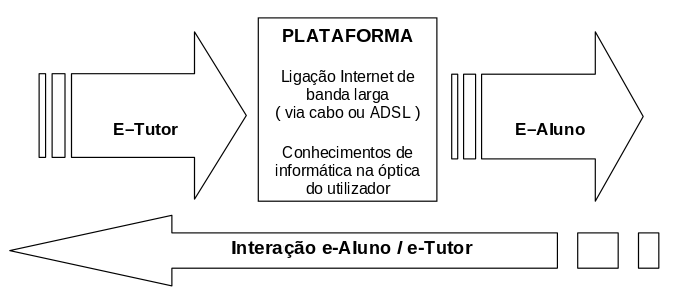
\includegraphics[keepaspectratio=true,scale=0.6]{figuras/e-learning-barbosa.png}
  \caption{Processo de \textit{e-Learning} por \citeonline{barbosa}}
\end{figure}

\par
É importante deixar claro que existem diferenças entre o \textit{e-Learning} e a EAD, enquanto a EAD é definido como qualquer ensino a distância, ou seja uma forma de educação em que o professor, conteúdo e aluno podem estar em locais e tempos diferentes, o \textit{e-Learning} é uma forma de Educação a distância que utiliza os meios tecnológicos como a Internet.


\subsubsection{AS VANTAGENS E DESVANTAGENS DO \textit{E-LEARNING}}
As principais vantagens do \textit{e-learning}, mostradas por \citeonline[p.~80]{hall} em seu artigo são: multiplicação dos pontos de treinamento, facilidade de acesso das informações, diminuição dos custos, remoção dos deslocamentos de funcionários, minimização do tempo usado em treinamentos, rapidez na atualização de conteúdos e definição do ritmo de aprendizagem pelo próprio aluno.
\citeonline[p.~5]{barbosa} aponta a flexibilidade e a disponibilização da informação em tempo real como uma vantagem importante do \textit{e-Learning}, assim o aluno consegue ter um tempo próprio para aulas, podendo acessar as aulas a qualquer hora e local.
\par
Segundo \cite[p.~6]{bernardo} no \textit{e-learning}, o sistema computadorizado ou o treinador podem detectar mais facilmente falhas ou dificuldades dos alunos e corrigi-las imediatamente, de modo que isso não afete negativamente o aprendizado.
\par
No entanto a alta robotização do treinamento pode gerar dificuldades tanto em alunos como em professores, por ser algo relativamente novo, não existem muitas pessoas com experiência para desenvolver aulas on-line. \cite[p.~6]{bernardo} aponta para o problema de que os alunos podem não se sentir à vontade para participar de aulas virtuais, porque acham muito importante o encontro físico entre alunos e professores na sala de aula.
\par
A plataforma também deve ser simples de manusear, para facilitar a interatividade, tendo o apoio do formador, para poder tirar dúvidas, partilhar informações e experiências. Se os alunos tiverem dificuldades em usar a tecnologia disponibilizada na plataforma, podem ter que dedicar mais tempo para aprender a usar a plataforma, do que o acesso ao seu conteúdo. \apud[p.~5]{barbosa}{choi}
\par
\Idem[p.~6]{barbosa} aponta também uma controvérsia da "ausência" de relação humana, o que pode gerar ou não isolamento por parte do aluno. Mesmo que o aluno possa estar sozinho no local de acesso, ele poderá ter a companhia dos colegas virtuais e até do professor.

\subsubsection{E-LEARNING APOIADO POR VÍDEOS}
O vídeo se tornou um recurso de fácil acesso, mais seu na educação somente começou a partir da década de 90, \citeonline{moran} foi um dos pioneiros a escrever sobre esse assunto no Brasil com o artigo "O Vídeo na Sala de Aula", no artigo o autor fala sobre as linguagens da TV e do vídeo, e também sobre seu impacto na comunicação.
\par
\citeonline[p.~3]{moran} destaca pontos importantes na utilização de vídeos na educação como: auxiliar o despertar da curiosidade, permite desenvolver cenários desconhecidos pelos alunos, proporciona simulações de realidade, reproduz também documentários, entrevistas, depoimentos e ajuda no desenvolvimento do senso crítico. Segundo \citeonline[p.~3]{moran}:
\begin{citacao}
  As tecnologias são pontes que abrem a sala de aula para o mundo, que representam, medeiam o nosso conhecimento do mundo. São diferentes formas de representação da realidade, de forma mais abstrata ou concreta, mais estática ou dinâmica, mais linear ou paralela, mas todas elas, combinadas, integradas, possibilitam uma melhor apreensão da realidade e o desenvolvimento de todas as potencialidades do educando, dos diferentes tipos de inteligência, habilidades de atitudes.
\end{citacao}

\section{SISTEMA DE GESTÃO DE APRENDIZADO (\textit{LMS})}

\citeonline[p.~2]{andrade} descreve o \ac{LMS} como um software que controla o desenvolvimento, gerenciamento e acompanhamento de cursos de aprendizagem online. O \ac{LMS} é um sistema de gestão que possui funcionalidades para suportar o aprendizado a distância tais como: distribuição, acompanhamento, monitoramento e administração de conteúdo de aprendizagem com os progressos e interações dos alunos.
\par
Segundo \citeonline[p.~3]{goni}:
\begin{citacao}
  Um \textit{LMS} tem como um dos objetivos, simplificar a administração dos programas de treinamento e ensino em uma organização. O sistema auxilia no planejamento dos processos de aprendizagem e ainda permite que os participantes colaborem entre si através da troca de informações e conhecimentos.
\end{citacao}
\par
Esses sistemas ajudam na disponibilidade das informações, análises, rastreamento de dados e a geração de relatórios sobre o andamento dos cursos.

As principais funcionalidades do sistema \ac{LMS}, são:
\begin{itemize}
  \item Criar e administrar cursos;
  \item Oferecer ferramentas de comunicação como listas de discussão, \textit{chats} e mensagens instantâneas;
  \item Administrar grades curriculares e listagens de espera;
  \item Fornecer tarefas, avaliações e exercícios;
  \item Monitorar o acesso do usuário;
  \item Administrar matrículas de aprendizes;
  \item Gerar relatórios e informações sobre o desempenho dos aprendizes, etc;
\end{itemize}

\subsection{\textit{MOODLE}}
O \ac{Moodle} (Ambiente de Aprendizagem Dinâmico Modular Orientado a Objetos), é um software livre criado pelo australiano Martin Dougiamas no ano de 1999, é um software de gerenciamento de cursos que auxilia os educadores a criarem cursos \textit{on-line}. Muito usado em cursos à distância por possuir funcionalidades que ajudam o professor no processo de avaliação além promover aprendizagem colaborativa. O \ac{Moodle} é um \textit{software} livre fornecido gratuitamente sobre a licença \textit{GNU Public License}\footnote{www.gnu.org/copyleft/gpl.html}. \cite{moodle}
\par
O \ac{Moodle} foi criado para ser compatível, flexível, é fácil de ser modificado. Foi escrito usando-se a linguagem \ac{PHP}, que o faz funcionar em qualquer plataforma de computador com um mínimo de esforço. Segundo o site oficial do Sistema, existem mais de 49 mil sites registrados com o sistema em 214 países \cite{moodle-stats}
\par
O motivo da adoção do sistema por varias organizações é a sua facilidade de instalação e atualização, ser livre, apresentar grande flexibilidade nas configurações e oferecer recursos tecnológicos uteis para a EAD.
\par
Uma das vantagens do \ac{Moodle} é a possibilidade do uso de padrões abertos como o \ac{SCORM} e o \ac{LTI} o que o torna uma plataforma é interoperável, permitindo a integração de aplicações externas e informações em uma única plataforma \ac{Moodle}.
\par
A plataforma é divida em blocos e módulos, como a maioria dos portais \textit{Web} conhecidos como \ac{CMS}. No entanto o \ac{Moodle} e categorizado como um \ac{LMS}. Utilizando essa arquitetura, novos módulos podem ser desenvolvidos de forma independente, e disponibilizados e utilizados de acordo com a necessidade.

\subsection{Padrões de \textit{E-Learning}}
Segundo a ISO, padrões são definidos como "acordos documentados que contém especificações técnicas ou outros critérios precisos que são usados como regras, guias ou definições de características de modo a garantir que materiais , produtos, processos e serviços sirvam a seus propósitos".
\par
Com o crescimento do uso do computador pessoal as tecnologias digitais vem aumentado na área da educação. Porem, essas tecnologias são desenvolvidas em formas divergentes, diversos cursos, módulos e sistemas desenvolvidos para fornecer os cursos, são criados independentemente um dos outros, geralmente isso gera mais custos e esforço, por que sem o uso de um padrão, um curso precisa ser desenvolvido diversas vezes para funcionar em vários \ac{LMS}.
\par 
Sem uma especificação de como os cursos devem ser feitos, os desenvolvedores da ferramenta, geralmente esperam que outros se conformem com sua própria estrutura dificultando assim a interoperabilidade entre os sistemas.
\par
Segundo \citeonline[p.~8]{bianco-standards}, existem quatro vantagens no desenvolvimento de cursos e ferramentas usando um padrão do \textit{e-learning}, são esses:
\begin{itemize}
  \item Durabilidade: Não é necessário realizar modificações na integração se a versão do \textit{software} mudar.
  \item Interoperabilidade: Funcionamento em uma grande variedade de sistemas para qual o padrão foi desenvolvido, como é o caso dos \textit{LMS}.
  \item Acessibilidade: Indexação e rastreamento sob demanda do conteúdo.
  \item Reusabilidade: Possibilidade de uso em diversas outras ferramentas.
\end{itemize}
\par
Para esse projeto, foram analisados dois dos mais conhecidos padrões de \textit{e-learning}, e escolhido o mais adequado para o caso de uso, os padrões \ac{SCORM} e o \ac{LTI}.

\subsubsection{\textit{SCORM (Shareable Content Object Reference Model)}}
O \ac{SCORM} teve a sua primeira versão lançada em 2000, pela \ac{ADL}, um consórcio de grupos internacionais em tecnologias educativas, liderado pelo Departamento de Defesa dos Estados Unidos, visando a pesquisa e criação de recursos para aprendizagem \cite{adl}.
\par
Segundo \citeonline[p.~24]{fernandes-scorm}, uma das grandes características do \ac{SCORM} é sua reutilização e interoperabilidade, dando independência da plataforma onde os objetos do SCORM podem ser usados, facilitando assim a migração dos cursos entre os diferentes \ac{LMS} compatíveis com esse modelo. O \ac{SCORM} é um conjunto de especificações para a disponibilização de conteúdos e serviços de aprendizagem pelo computador e a \ac{WEB} \cite{adl}.
\par
A especificação do \ac{SCORM} está dividido em 4 documentos, chamados de livros pela \cite{adl}, são eles:
\begin{enumerate}
  \item \textbf{\textit{The Scorm Overview}}: Descreve o \ac{SCORM} em geral, definindo seus conceitos sobre o modelo.
  \item \textbf{\textit{The SCORM content Aggregation Model (CAM)}}: Descreve os componentes usados em uma interação de aprendizagem, mostrando como empacotar os cursos e realizar a migração entre os ambientes de aprendizagem, descreve também os metadados que precisam ser usados na descrição do objeto de aprendizagem.
  \item \textbf{\textit{The SCORM Run-Time Enviroment (RTE)}}: Trata da execução dos objetos criados no modelo \ac{SCORM}, por exemplo, como é feita a comunicação do objeto com o ambiente de aprendizagem.
  \item \textbf{\textit{The SCORM Sequencing and Navigation (SN)}}: Trata do navegação do conteúdo do objeto de aprendizagem, descrevendo como deve ser feita a navegação atravès do conteúdo do objeto construído.
\end{enumerate}

\begin{figure}[h]
  \centering
  \label{fig:scorm-funcionamento-dutra}
  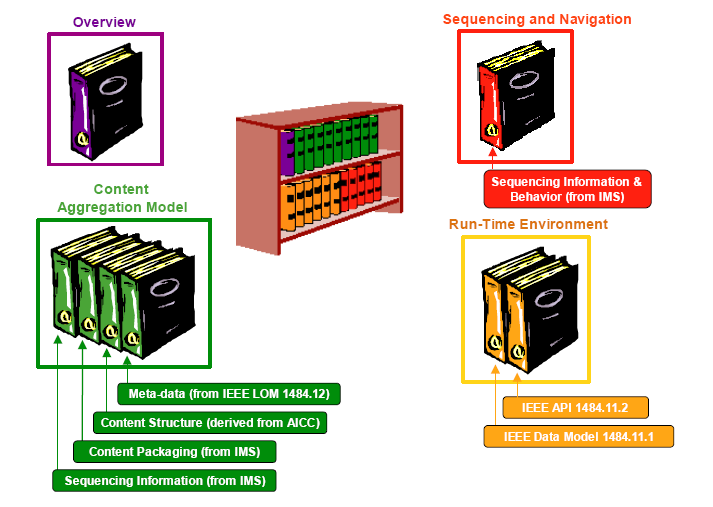
\includegraphics[keepaspectratio=true,scale=0.7]{figuras/scorm-funcionamento-dutra.png}
  \caption{SCORM como conjunto de especificações. Fonte: \citeonline{dutra-scorm-ims}}.
\end{figure}
\par
O pacote \ac{SCORM} gerado tem como resultado um arquivo \textit{ZIP}, esse arquivo contem o conteúdo do curso, e também deve possuir todos os arquivos \textit{HTML}, \textit{Javascript}, imagens e animações, além de um arquivo de manifesto chamado \textit{imsmanifest.xml}. Este arquivo descreve a estrutura lógica do conteúdo como a navegação das páginas e a organização de todo conteúdo. O \ac{LMS} carrega esse pacote e então cria o relacionamento entre as unidades (Pacote \textit{SCORM} e o \textit{LMS}). \cite[p.~39]{fernandes-scorm}.
\par
Como o \textit{SCORM} e distríbuido como um pacote \textit{ZIP}, permite que os seus conteúdos resistam a evolução tecnológica, com custo baixo de reconfiguração, esse pacote pode ser reaproveitado em \textit{LMS} compatíveis com seu funcionamento inalterado.

\subsubsection{\textit{LTI (Learning Tool Interoperability)}}
O \textit{LTI} foi criado pela \textit{IMS}, a primeira versão TI 1.0 foi lançado em 2006 mais na epoca foi considerado muito complexo, e não teve uma boa adoção. O projeto do \textit{Learning Tools Interoperability} foi desenvolvido com os mesmos objetivos do TI, mais com uma solução mais simples. \cite{ims}
\par
A versão atual do \textit{LTI} é a 1.1, que suporta dados de retorno ao \textit{LMS} como as notas que ao aluno atingiu no curso.
\par
\begin{citacao}
  O \textit{LTI} tem a habilidade de fornecer á um usuário em um \textit{LMS} (Ou outro sistema \textit{web} com suporte ao padrão) de acessar uma aplicação de aprendizagem separada, um item de conteúdo protegido ou outro recurso restrito. \cite[p.~2, tradução nossa]{vickers-ims}
\end{citacao}
\par
Quando um usuário que está em um \textit{LMS} para um sistema com suporte ao \textit{LTI} alguns dados são enviados juntos a ele:
\begin{itemize}
    \item Detalhes sobre ele (como nome e email);
    \item Detalhes sobre o contexto institucional (como o nome do \textit{LMS que está sendo usado, nome da faculdade});
    \item Detalhes do contexto de onde o usuário está vindo (como o curso especificado);
    \item A sua função no \textit{LMS} (como professor ou aluno);
\end{itemize}
Esses dados são fornecidos pelo próprio \textit{LMS}, no seu lançamento.
\par
O lançamento do sistema externo ocorre de maneira segura (usando \textit{OAuth}) pelo navegador do usuário. Uma conexão e criada entre esses dois sistemas por meio de autenticação, as únicas informações que o \textit{LMS} precisa sobre o sistema externo são:
\begin{itemize}
    \item A \ac{URL} do sistema;
    \item Uma chave para identificar o cliente (chamada de \textit{"consumer key"} ou chave do cliente);
    \item Uma outra chave secreta para proteger a conexão;
\end{itemize}
\par
Segundo \citeonline[p.~2]{vickers-ims} o sistema de Gestão de Aprendizagem (\textit{LMS}), na especificação do \textit{LTI}, é chamado de \ac{TC} em português seria algo como "Consumidor da Ferramenta", que é o sistema que irá "consumir" a outra aplicação ou recurso, que e provido pelo \ac{TP} em português "Provedor da Ferramenta".
\par
Um \textit{TP} pode ser tanto um \textit{LMS} como um portal empresarial, ou qualquer sistema que suporte a implementação do \textit{LTI}. É um \textit{TC}, pode ser um \textit{Wiki} (Um site de edição coletiva) ou uma ferramenta de questionários por exemplo.
\begin{figure}[h]
    \centering
    \label{fig:ims-lti-funcionamento}
    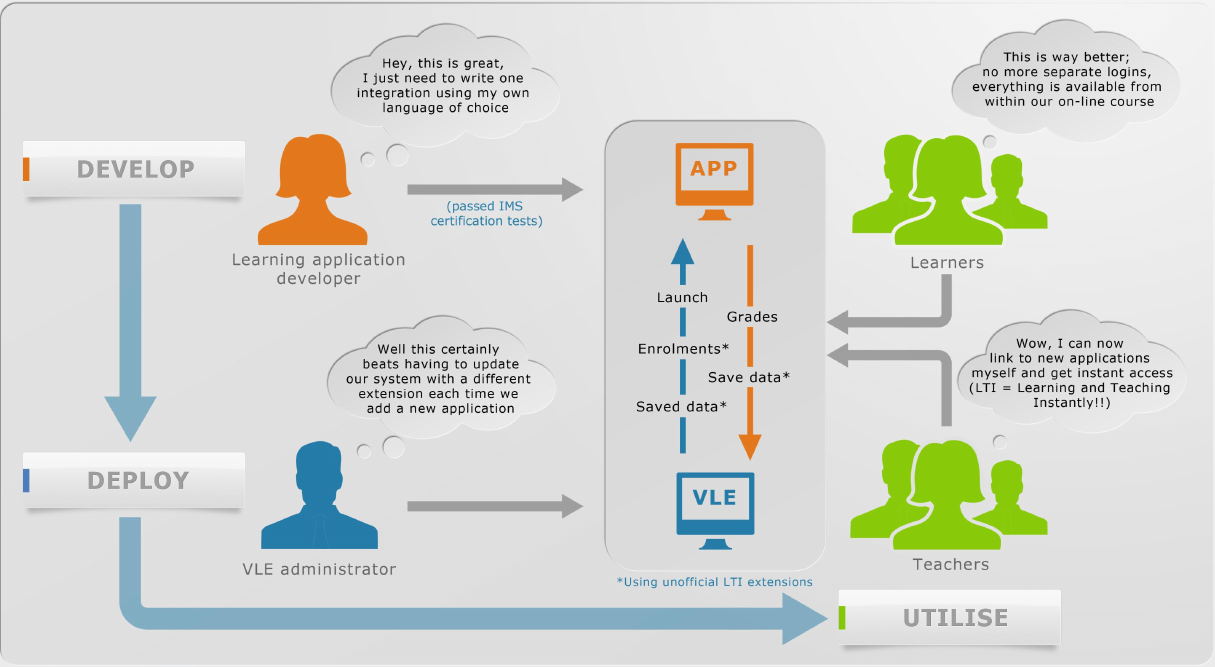
\includegraphics[keepaspectratio=true,scale=0.5]{figuras/ims-lti-funcionamento.png}
    \caption{Funcionamento do \textit{LTI}. Fonte: \citeonline{ims}}
\end{figure}
